
% Inbuilt themes in beamer
\documentclass{beamer}

\usetheme{Singapore}
\definecolor{mycolor}{RGB}{208,208,237}
\usepackage{graphicx} % Allows including images

\addtobeamertemplate{navigation symbols}{}{%
	\usebeamerfont{footline}%
	\usebeamercolor[fg]{footline}%
	\hspace{1em}%
	\insertframenumber/\inserttotalframenumber
}

\setbeamercolor{footline}{fg=blue}
\setbeamerfont{footline}{series=\bfseries}

%% Title page details: 
%\title{\Huge \textbf{Mid-Term Presentation} \\
%\large FEM and its application to static structures}
%\author{\textbf{Group A:}\\
%\footnotesize{Samrajya Raj Acharya , 1\\
%Bishesh Kafle , 9\\
%Priyanka Panta , 13\\
%Mukesh Tiwari, 22}}
%
%\logo{
\includegraphics[width=2cm]{logo.png}}
%
%
%\begin{document}
%
%
%% Title page frame
%\begin{frame}
%    \titlepage 
%\end{frame}

\title{\Huge Mid-Term Presentation}
\titlegraphic{
\includegraphics[height=3cm]{logo.png}}
\subtitle{FEM and its application to static structures}
\author{Group A}

\setbeamercolor{title}{bg=mycolor,fg=black}

\makeatletter
\setbeamertemplate{title page}
{
	\vbox{}
	\vfill
	\begin{centering}
		\begin{beamercolorbox}[sep=8pt,center]{title}
			\usebeamerfont{title}\inserttitle
		\end{beamercolorbox}
		\setbeamercolor{title}{bg=white,fg=black}
		\vspace{20pt}
		\begin{beamercolorbox}[sep=8pt,center]{title}
			{\usebeamercolor[fg]{titlegraphic}\inserttitlegraphic\par}
			\vskip1.25em%
			\ifx\insertsubtitle\@empty%
			\else%
			\vskip0.25em%
			{\usebeamerfont{subtitle}\usebeamercolor[fg]{subtitle}\insertsubtitle\par}%
			\fi%     
		\end{beamercolorbox}%
		\vskip1em\par
		\begin{beamercolorbox}[sep=8pt,center]{author}
			\usebeamerfont{author}\insertauthor
		\end{beamercolorbox}
		\vskip-1em\par % change here
		\begin{beamercolorbox}[sep=8pt,center]{institute}
			\usebeamerfont{institute}\insertinstitute
		\end{beamercolorbox}
%		\begin{beamercolorbox}[sep=8pt,center]{date}
%			\usebeamerfont{date}\insertdate
%		\end{beamercolorbox}\vskip0.5em
	\end{centering}
	\vfill
}
\makeatother

\begin{document}
	
	\maketitle

% Remove logo from the next slides
\logo{}

%--BISHESH 

\part{}
\section{Introduction}
\begin{frame}{Introduction}
	\begin{itemize}
		\item  Finite Element Method (FEM) is a procedure of numerical solution of a domain viewed as the collection of sub-domains.
		\vspace{0.6cm}
		\item FEM on static structures computing the stress and displacement.
		\vspace{0.6cm}
		\item The actual problem will be replaced by simpler ones to find one approximate solution. 
	\end{itemize}
	
\end{frame}


\section{Progress}
\begin{frame}{Gantt Chart : Progress}
	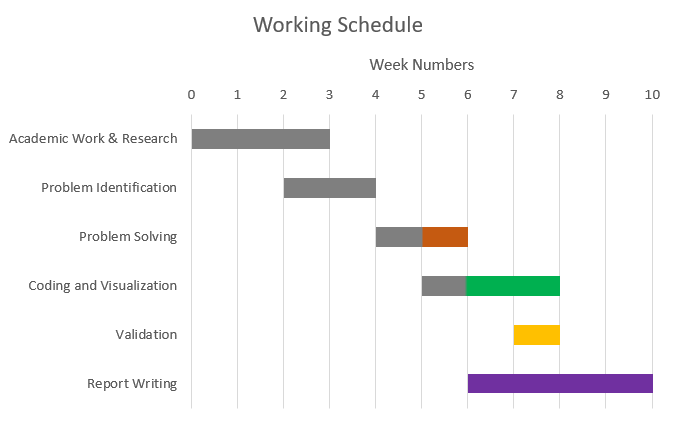
\includegraphics[width = 10cm, height = 6cm]{progress.png}
\end{frame}

%---PRIYANKA


\begin{frame}[t]{Progress so far.}
	\begin{itemize}
		\item \textbf{Problem Identification}\\
			each member came up with various problems where FEM is used and we decided on trusses.
			
				\item \textbf{Theoretical Background}\\
			Went through basic ideas about FEM and the new concepts.
		\end{itemize}

\end{frame}

\begin{frame}[t]{Progress so far. }
	\begin{itemize}
		\item \textbf{Manual and Python Implementation}\\
		wrote custom classes and procedures for solving the problem in python. Tested code against examples in book and worked on  debugging.
		
		\item \textbf{Visualization}\\
		Worked on visualizing the structure and the deformations in python using the problem data and solution data.\\
		
	
	\end{itemize}
	
\end{frame}


\begin{frame}
	\begin{exampleblock}{\textbf{\color{black}{\large{Class Implementation}}}}
		custom classs in jupyter notebook for nodes and matrices.
		
		
	\end{exampleblock}\vspace{20pt}
	
	
	
	\begin{block} {\textbf{\color{black}{\large{Mechanical Approach}}}}
		followed joint and sectional method and verified .
	\end{block}\vspace{20pt}
	
	\begin{block}{\textbf{\color{black}{\large {Visualization}}}}
		code for visualizing any problem given the coordinates.
		
	\end{block}
	
\end{frame} 

%---SAMRAJYA
\section{Upcoming}
\begin{frame}{Future Plans}
	
	Working of solution:
	\begin{itemize}
		\item Solution part is working for some problem but not for all.
		\item Why, how and in which cases the solution can work in all problem is to be worked on.
		
	\end{itemize}
	
	Software Visualization:
	\begin{itemize}
		\item Data has been generated, solved upon and visualized to an extent both theoretically and manually.
		\item The streamlining of all these components and compiling it is needed.
		
	\end{itemize}
	
\end{frame}

% Lists frame

\begin{frame}{Things left}
	
	Theoretical readings:
	\begin{itemize}
		\item As of now, we have only worked and implemented on software.
		\item Knowledge of mandatory principles and applications of FEM is to be thoroughly studied.
		
	\end{itemize}
	
	Report Writing:
	\begin{itemize}
		\item Final report of the project is to be written.
		
		
	\end{itemize}
	
\end{frame}

\part{}
\begin{frame}
	\centering \Large
	\emph{Thank You}
\end{frame}


\end{document}
